\subsection{Aktivitetsdiagram}


\subsubsection{Registrering}
Inden app'en anvendes første gang, skal KOL-patienter registreres som brugere af systemet. Dette skal foregå i forbindelse med rehabiliteringsforløbet, hvor sundhedspersonale opretter patienterne i en database. Patienterne får tilknyttet et medlemsID bestående af tal, der identificere lokalisation, årstal og måned for påbegyndt rehabilieringsforløb samt nummerering af den enkelte KOL-patient. Et eksempel på dette kan være 01-2017-03-01. 

Sundhedspersonalet opretter nye patienter i databasen ved følgende.....

\subsubsection{Log ind}
Når KOL-patienten vil anvende app'en skal medlemsID eller brugernavn samt kodeord indtastes. Systemet sender det indtastede medlemsID eller brugernavn til databasen, som tilbagesender det tilhørende kodeord, hvis det findes i databasen. Hvis de indtastede informationer ikke findes i databasen sendes en fejlmeddelelse i form af 0. Systemet sammenligner herefter brugerens indtastede kodeord med den returnerede værdi fra databasen. Er de to værdier ens, har brugeren indtastet korrekte informationer sender databasen brugerdata og viser app'ens menu. Er de to værdier ikke ens, tilbagesender systemet en fejlmeddelelse og brugeren får derefter mulighed for at indtaste informationer igen. Aktivitetsdiagrammet over log ind fremgår af  \autoref{fig:logind}.

\begin{figure} [H]
\centering
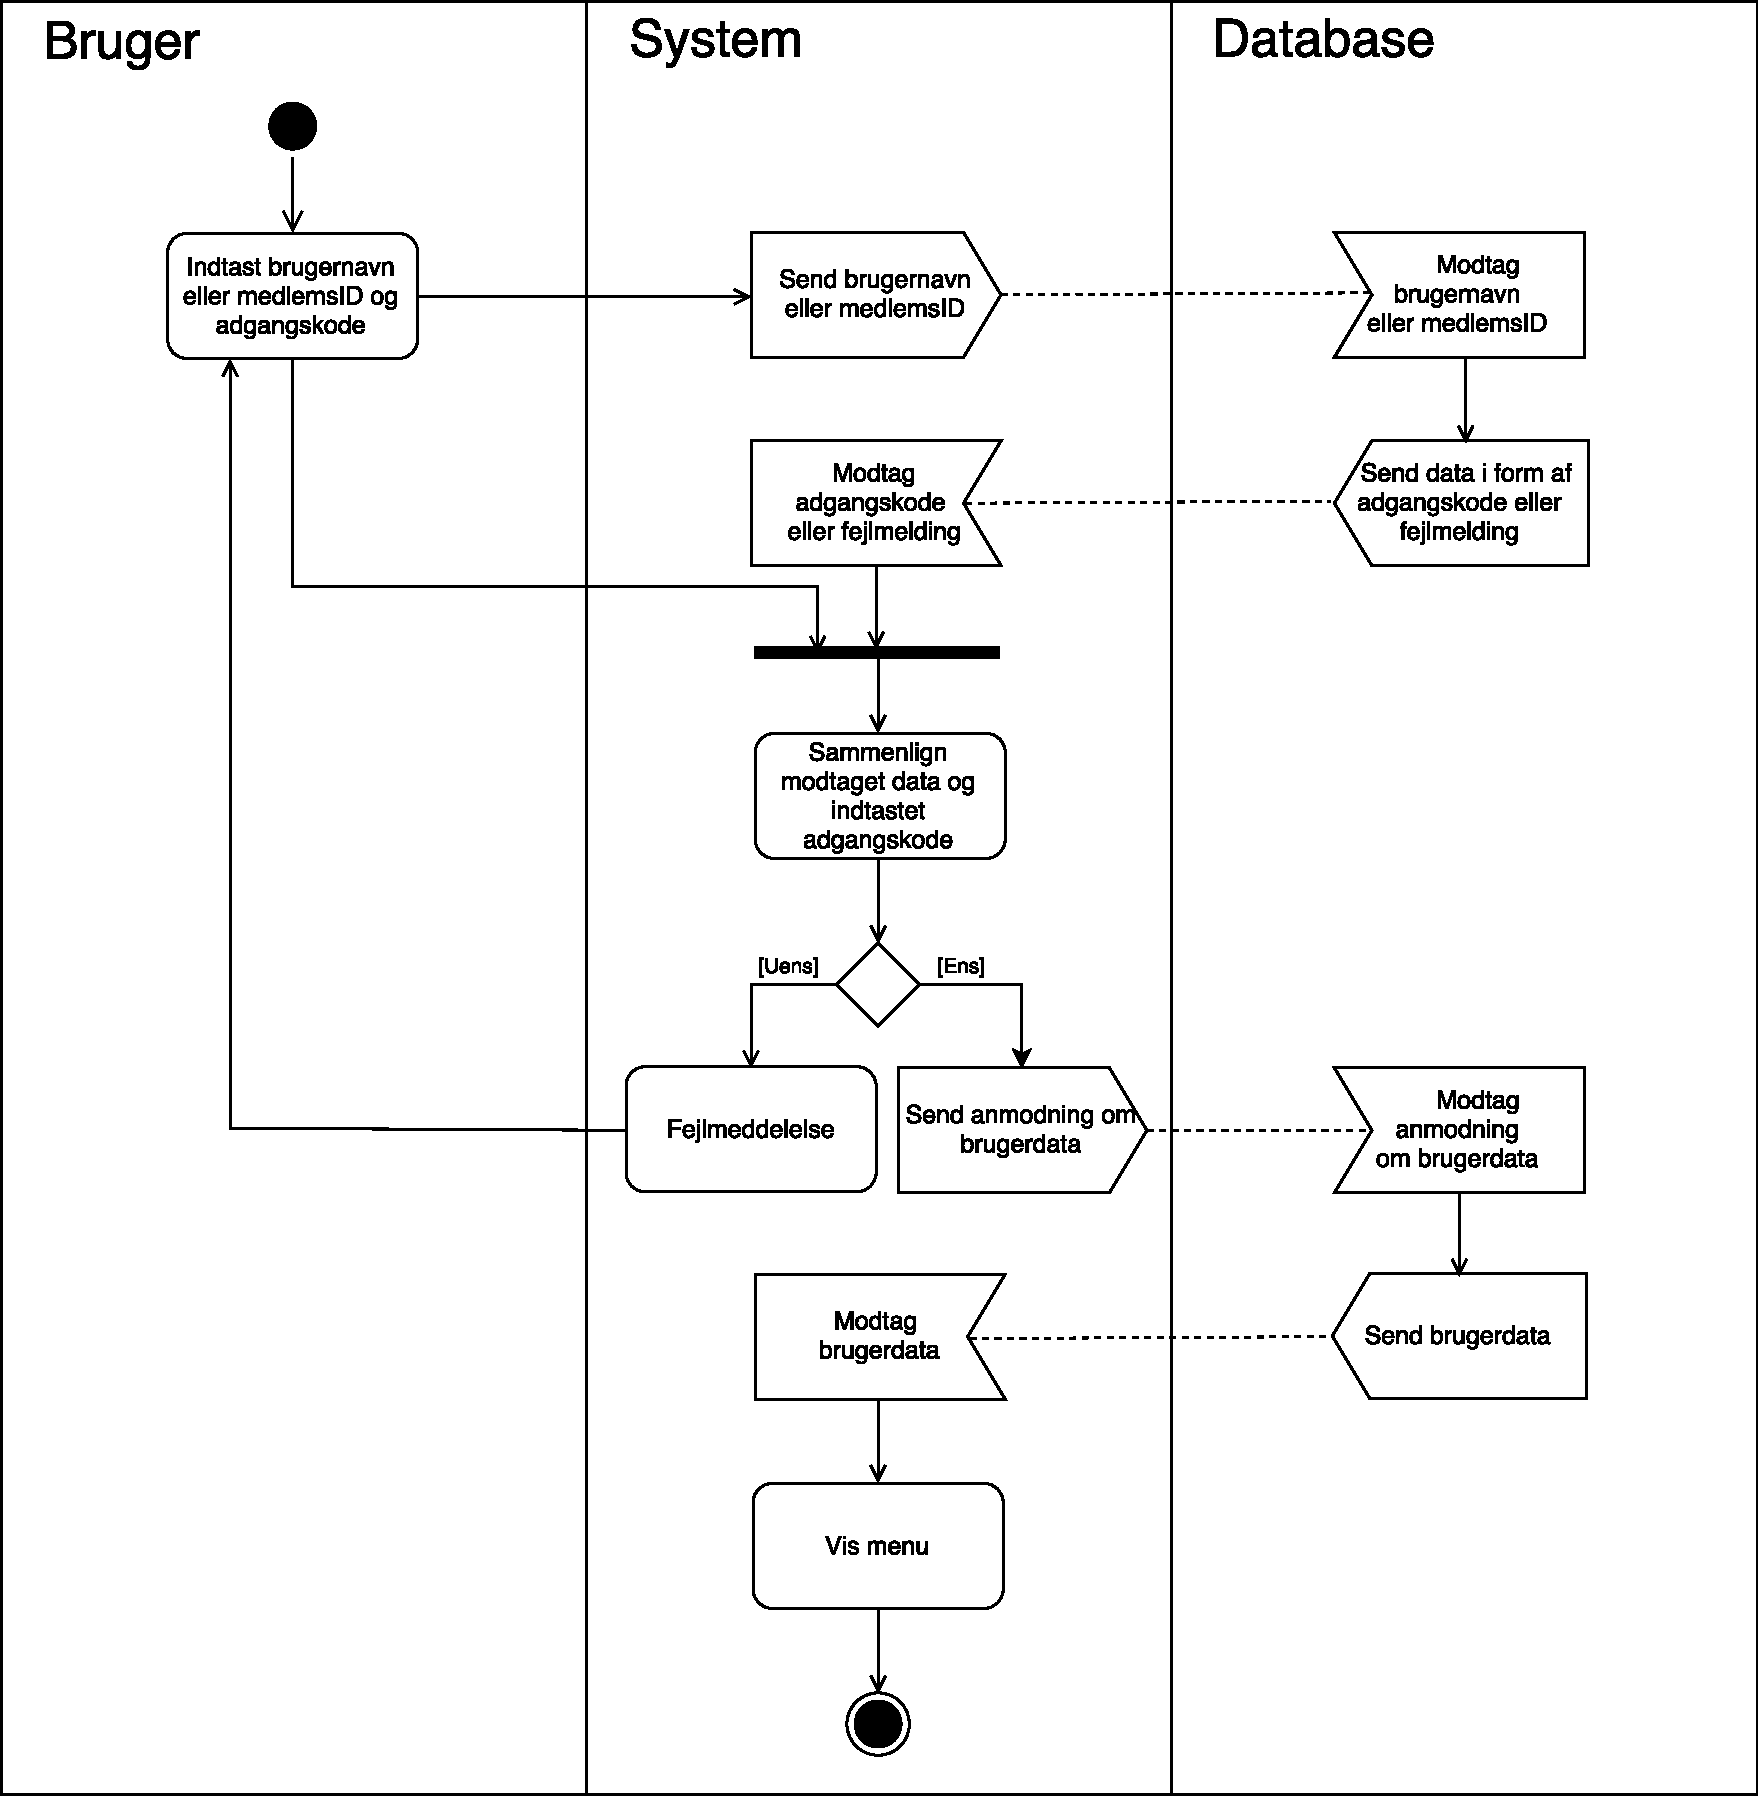
\includegraphics[width=0.9\textwidth]{figures/aktivitetsdiagram/Logind}
\caption{Aktivitetsdiagram over log ind.}
\label{fig:Logind}
\end{figure}



